\chapter{Přístrojové vybavení}
\label{sec:instruments}
Na úvod experimentální části je vhodné popsat konkrétní přístroje
a~další součásti používané při pokusech,
neboť některé se opakují ve více aparaturách.

\section{Laser Ekspla \instrname{PL2231-50}}
\label{sec:instruments-laser}
Ústřední součástí všech prováděných pokusů byl samozřejmě laser.
Vždy bylo použito totéž zařízení, konkrétně model \instrname{PL2231-50}
od firmy Ekspla.
Je to diodou čerpaný pevnolátkový pikosekundový laser typu Nd:YAG
poskytující velmi krátké pulzy záření o~vysokém okamžitém výkonu.
Délka pulzu (FWHM) činí \SI{29}{\pico\second}
a~jejich energie může dosahovat až \SI{30}{\milli\joule},
což představuje okamžitý výkon v~řádu \si{\giga\watt}.
Pulzy se opakují s~frekvencí \SI{50}{\hertz}.

\begin{figure}[htp]
	\centering
	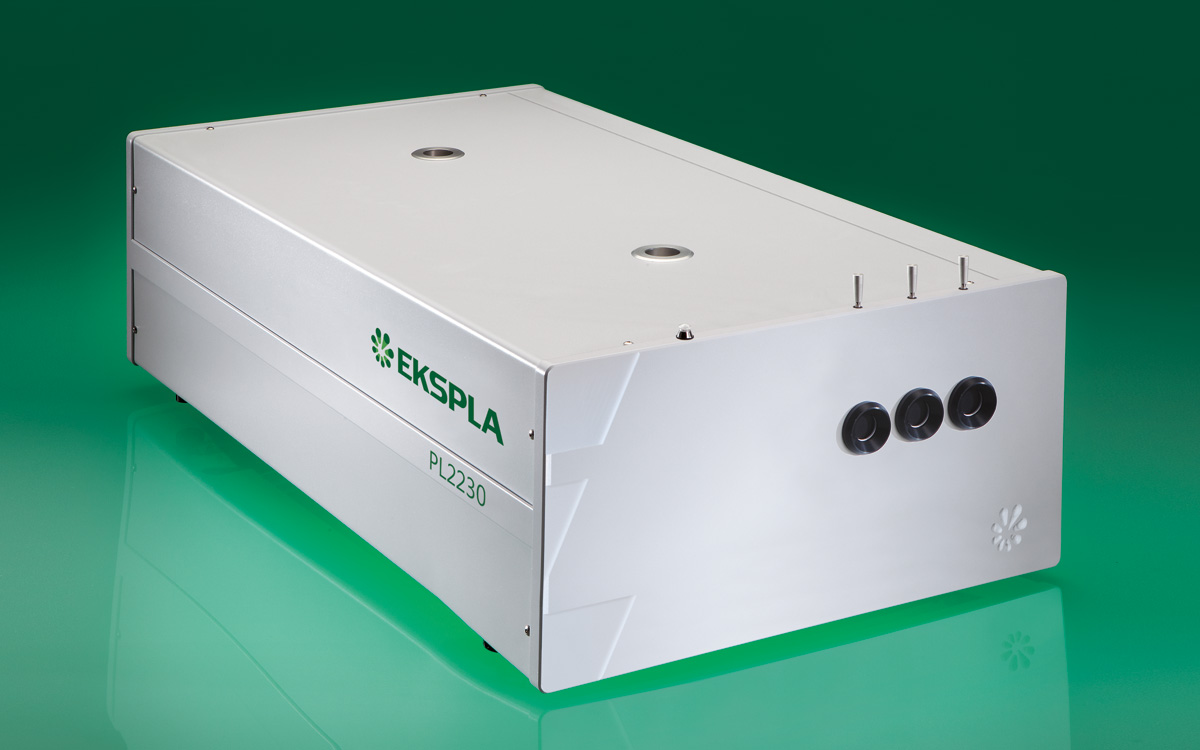
\includegraphics[width=\textwidth]{laser}
	\caption{Pikosekundový laser Ekspla (fotografie z~katalogu).
		Použitý model je ze stejné řady.
		Převzato z~\cite{ekspla-datasheet}.}
	\label{fig:instruments-laser}
\end{figure}

Aktivním médiem je krystal yttrito-hlinitého granátu (\ce{Y3Al5O12})
dopovaný ionty neodymu (\ce{Nd3+}).\autocite{wiki-ndyag}
Základní vlnová délka laseru je \SI{1064}{\nano\metre},
stejně jako pro všechny lasery typu Nd:YAG,
jeho součástí jsou ale teplotně stabilizované jednotky obsahující
krystaly di\-hydro\-gen\-fosfo\-rečnanu draselného (KDP a~KD*P),
které umožňují generování druhé, třetí a čtvrté harmonické frekvence,
tedy vlnových délek \SIlist{532; 355; 266}{\nano\metre}.
\autocite{ekspla-datasheet}

Generování začíná v~hlavním pevnolátkovém oscilátoru čerpaném diodami,
který vytváří řetězce pulzů s~frekvencí opakování jednotlivých pulzů
přibližně \SI{87}{\mega\hertz} (tzv.~\emph{trains}).
Pulzy jsou slabé, jejich energie se pohybuje v~jednotkách \si{\nano\joule}.
Tyto putují do diodového regenerativního zesilovače se zesílením v~řádu $10^6$
a~poté do víceprůchodového výkonového zesilovače,
takže jejich konečná energie je kolem $\SI{30}{\milli\joule}$.
Výstupní energie je nastavitelná v~krocích po zhruba \SI{1}{\percent}
a~je velmi stabilní mezi po sobě jdoucími pulzy
(odchylky jsou menší než \SI{0.5}{\percent} středního kvadratického průměru
při nastavené základní vlnové délce).
\autocite{ekspla-datasheet}

Výstupní svazek je z~\SI{99}{\percent} svisle polarizovaný.
Jeho profil je podle výrobce přibližně gaussovský
(viz obrázek~\ref{fig:instruments-beamprofile})
o~průměru cca \SI{6}{\milli\metre} na úrovni $1/e^2$ maxima
pro vlnovou délku \SI{1064}{\nano\metre}.
\autocite{ekspla-datasheet}
Navzdory těmto specifikacím se ukázalo, že profil svazku je závislý
na nastavené energii pulzu v~míře, kterou nelze zanedbat.
Tato problematika je podrobněji popsána v~dalších kapitolách,
viz především oddíl \ref{sec:lif-rayleigh}.

Laser je vybaven vlastním měřičem, který průběžně zaznamenává energii pulzu.
K~synchronizaci dalších zařízení slouží spouštěcí signál s~nastavitelným
předstihem.\autocite{ekspla-datasheet}

\begin{figure}[htp]
	\centering
	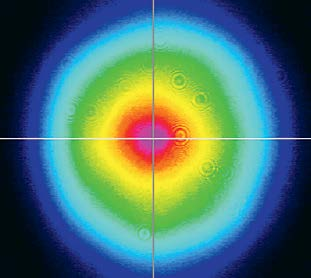
\includegraphics[scale=0.5]{ekspla-beamprofile}
	\caption{Typický profil laserového svazku v~blízkém poli
		uvedený v~technickém listu laseru.
		Převzato z~\cite{ekspla-datasheet}.}
	\label{fig:instruments-beamprofile}
\end{figure}

\section{ICCD kamera \instrname{Pimax}}
\label{sec:instruments-iccd}

\begin{figure}[htp]
	\centering
	\input{img/cameraeff}
	\caption{Kvantová účinnost kamery deklarovaná výrobcem.}
	\label{fig:instruments-cameraeff}
\end{figure}
